\section{Introduction}
% Placeholder~\cite{liu2022title2vec,liu2020ipod,liu2020epic30m,liu2021crisisbert,liu2020strategic,mu2022clustering,singhal2021analyzing}

% 大纲
% \begin{itemize}
%     \item Context of the problem (multi-lingual, multi-turn conversation intent classification: why is it important / significance of the problem
%     \item Challenges of the problem (1, 2, 3..)
%     \item Proposed solutions (for each problem). Intuition behind the proposal

%     \item Brief discussion on the various experiments and results
%     \item Impact of the solutions, if any
%     \item Summary of main contributions
% \end{itemize}



% Proposes solutions
% 1 & 3. Hard to improve acc for multi-turn intent recognition task in industry scenario, especially for multi-lingual scenario

% solution: 1. Fintune LLM with auto-generated dataset (shorten intent/cross-lingual label); solution: 2. RAG with original classifier address lower acc on multi-lingual and multi-turn intent recognition task.

% 2. Collecting dataset is a time-consuming task (Difficulty for dataset collection)
% solution: Proposed an HMM-based method to generate multi-turn data to improve acc on the first methods. The methods can also generate evaluation dataset on this task


% 1. Lower acc due to the longer and various (large variety) intent
% solution: Fintune LLM with auto-generated dataset (shorten intent/cross-lingual label);
% 2. How to improve the acc on this task for multi-lingual scenario
% solution: RAG with original classifier 

% \begin{itemize}
%     \item 1. Background of multi-turn text classification and LLM for text classification
%     \item 2. Briefly describe challenge of the task
%     (1) Lower acc due to the longer and various (large variety) intent; our solution: Fintune LLM with auto-generated dataset (shorten intent/cross-lingual label); (2) How to improve the acc on this task for multi-lingual scenario; solution: RAG with original classifier 
%     \item 3. Our contribution
% \end{itemize}

% Two challenges: 
% 1) length and numbers of intents -> LLM fine-tuned with compressed generation and cross-lingual label
% 2) but multi-turn annotation data is hard to collect so we developed LARA to reduce the dependence of multi-turn annotation data only need smaller model trained with single-turn training data  


A chatbot is an essential tool that automatically interacts or converses with customers. It plays a crucial role for international e-commerce platforms due to the rising consumer demand for instant and efficient customer service. Chatbots represent a critical component of dialogue systems \cite{weld2021survey} that can answer multiple queries simultaneously by classifying intent from the user's utterance to reduce waiting times and operational costs. Naturally, the interaction with users could turn into a multi-turn conversation if they require more detailed information about the query. Developing an intent classification model for a dialogue system is not trivial, even if it is a typical text classification task. As we must consider contextual factors such as historical utterances and intents, failing to understand session context while recognizing user intention often leads to visible errors. It would invoke a completely wrong application or provide an unrelated answer \cite{6853573}. As a result, it faces several challenges in dialogue understanding.  

\begin{figure*}[t]
    \centering
    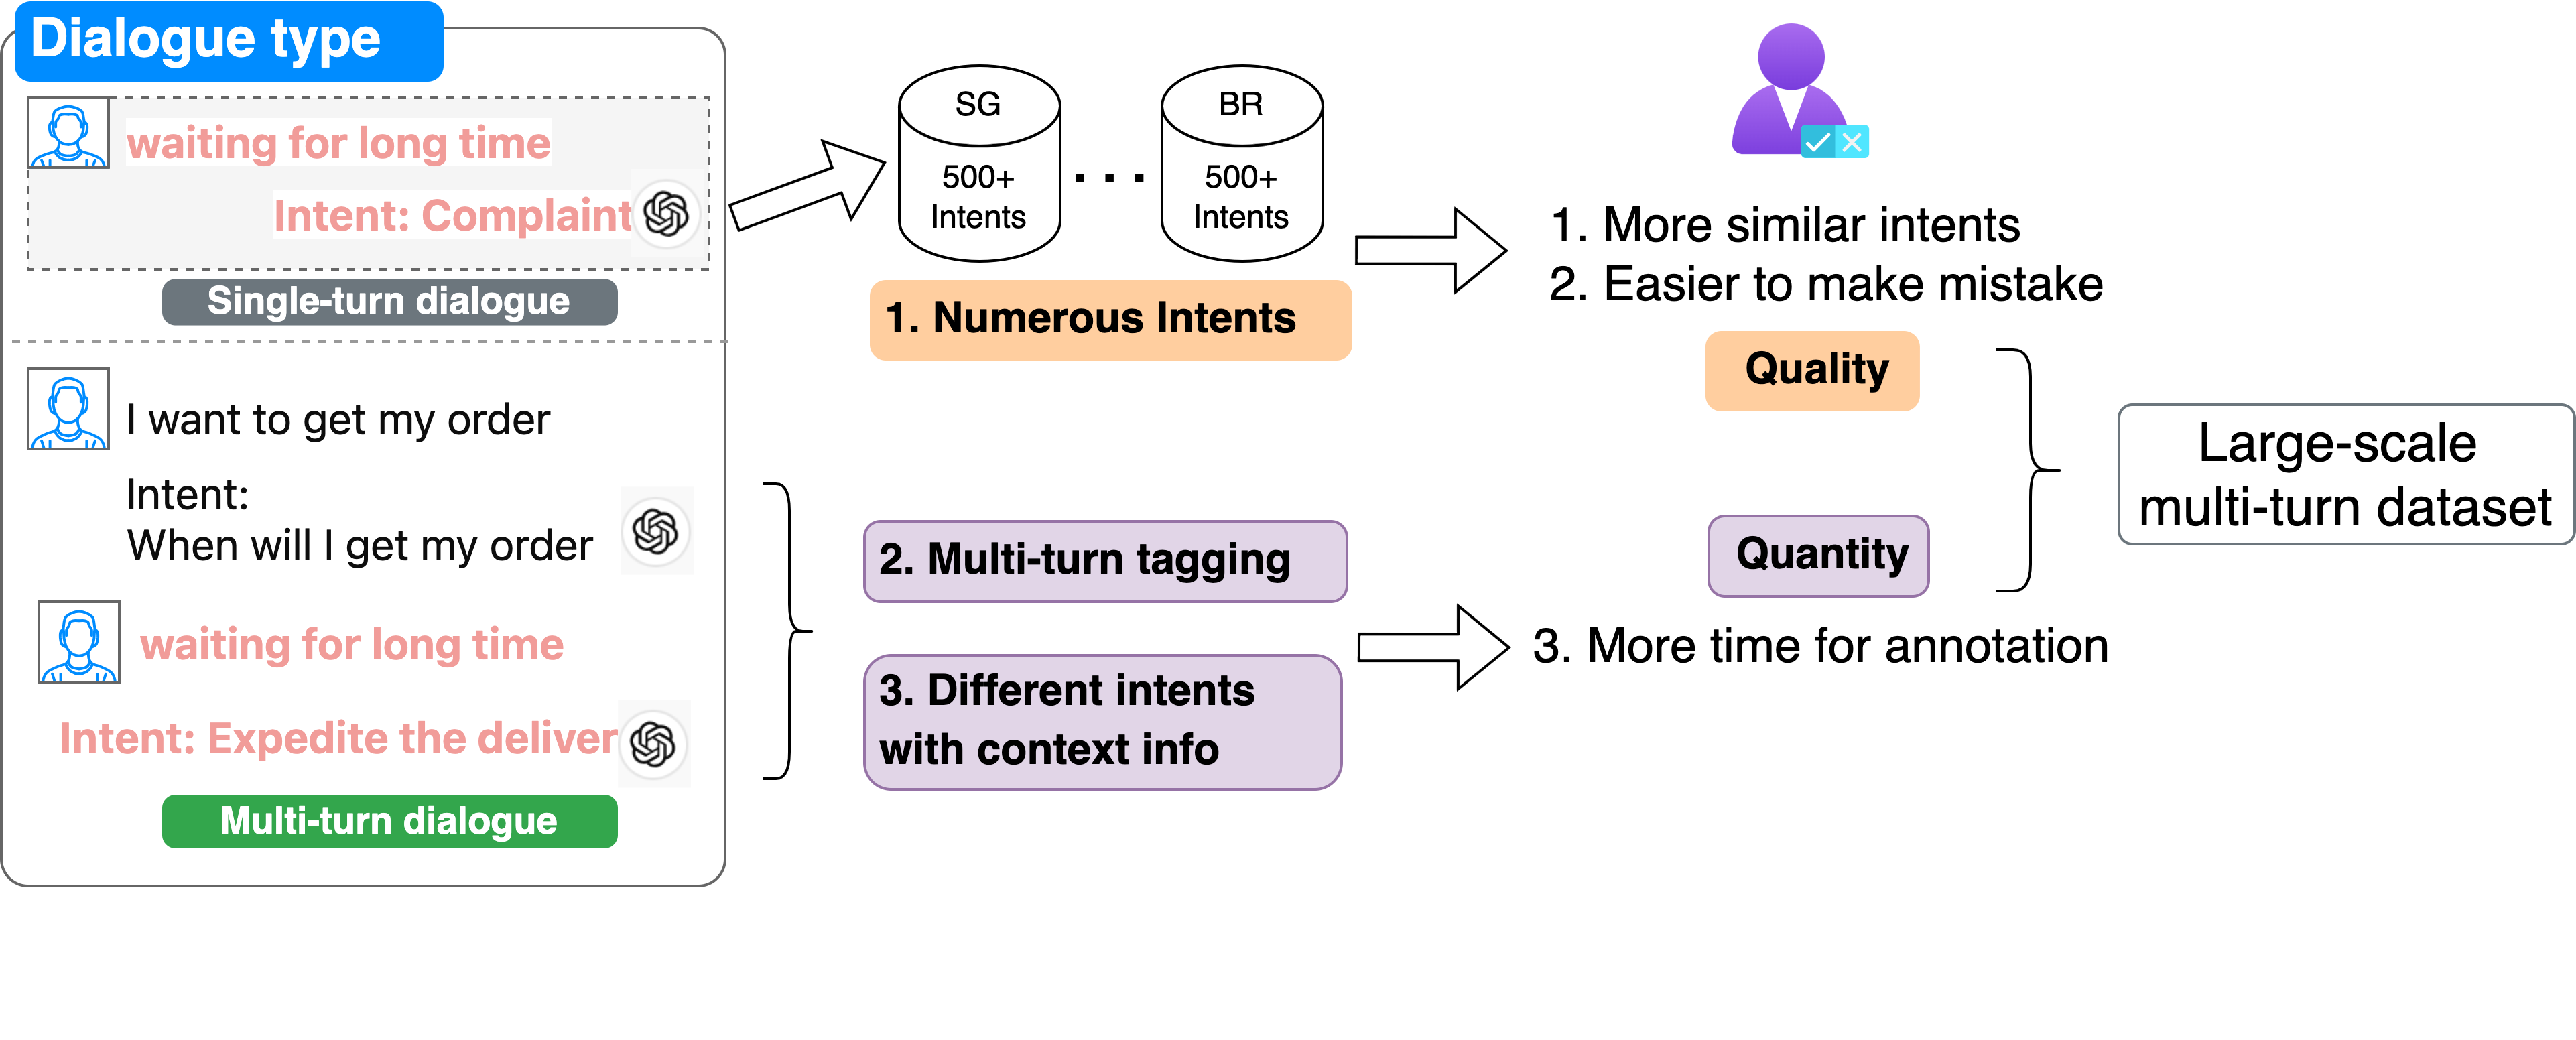
\includegraphics[width=.95\textwidth]{Figures/Challenge-for-multi-turn-dialogue.png}
    \vspace{-1cm}
    \caption{Annotation pipeline of multi-turn intent classification dataset }
    % \caption{Annotation pipeline of multi-turn intent classification dataset - a challenging task as there are hundreds of intents within the knowledge base of a chatbot to cover users' specific intents for each market. Furthermore, the complexity of classification increases as the number of market increases. }
    \label{fig:challenges}
    \vspace{-0.3cm}
\end{figure*}

The biggest challenge is that multi-turn datasets are hard to collect. %Some studies have already been done on this problem of 
While there are some studies on dialogue understanding in multi-turn intent classification~\cite{9082602,wu2021contextaware,Qu_2019}, they are made under the assumption of the availability of multi-turn training data, which is usually not the case in the real world. 

Figure~\ref{fig:challenges} shows the annotation pipeline of multi-turn intent classification. Unlike emotion recognition in conversation (ERC) with only less than 10 classes or topic classification within dialogue state tracking (DST) with tens of topics, there are hundreds of intents within the knowledge base of a chatbot to cover users' specific intents in each market, which increases the complexity of classification tasks and multi-turn data annotation. Annotators can easily make mistakes and spend more time making decisions due to the numerous intents. Combined, these make it a high-cost and time-consuming annotation task, and it is unrealistic to annotate large-scale multi-turn datasets manually. However, the performance will most likely suffer without enough training sample size. This calls for a more efficient method in solving the challenge \cite{Mo2023LearningTR}. 

%In this paper, we first study the feasibility of using LLM for supervised fine-tuning (SFT) to perform multi-turn intent classification using a generative method. Various intents increase the complexity of this task since the more tokens a large language model(LLM) generates, the lower the task performance \cite{rust2021good}. To conquer this, we showed two techniques: 1) compressed generation and 2) cross-lingual label, which help to reduce the difficulty of multi-turn classification tasks using the LLM generative method. 


%When building a transnational application, we also need to cope with the language understanding of different markets. Besides, there are also distinct intent sets which are catered to the local business operations, and the intents are ever changing over the course of business. Manually annotating and maintaining large scale multi-turn dataset is simply unrealistic. 

To tackle the above challenge, we propose \textbf{L}inguistic-\textbf{A}daptive \textbf{R}etrieval-\textbf{A}ugmentation, or LARA, which offers a pipeline of techniques to adopt only single-turn training data to optimize multi-turn dialogue classification. LARA first leverages an XLM-based model trained on single-turn classification datasets for each market, thus simplifying data construction and maintenance. Subsequently, LARA advances the field by selecting plausible candidate intents from user utterances and employing a retriever to gather relevant questions for prompt construction. This process facilitates in-context learning (ICL) with multi-lingual LLMs (MLLMs), significantly enhancing model efficacy without requiring market-specific multi-turn models.

% Firstly, we trained an XLM-based model on our single-turn classification dataset of each market, which is easier to construct and maintain. Secondly, the model can classify plausible candidate intents from all utterances from the user side. Then we adopt a retriever to collect 9 most similar questions under those candidate intents. Finally, we construct prompts based on them  and feed them into multi-lingual LLM (MLLM). With MLLM, we also relax the requirement to train multi-turn models for each market. 

In summary, the contributions of this paper are as follows:

%In this method  using LLM through in-context learning (ICL) in a zero-shot setting. To overcome the context limit of LLMs involving many intents, we introduced a way to retrieve highly plausible candidate intents using a single-turn model, which also helped filter noises for in-context learning.

\begin{enumerate}
  \item We introduce LARA as a multi-turn classification model only leveraging single-turn datasets to effectively address multi-turn data collection issues. 
  \item We conduct experiments on our e-commerce multi-turn dataset across six languages. LARA achieves state-of-the-art results and reduces inference time during ICL with MLLMs.
\end{enumerate}
